\documentclass[UTF8,8pt]{ctexart}
\usepackage{../template/Notes/notes}
\usepackage{multicol}
\setlength{\premulticols}{1pt}
\setlength{\postmulticols}{1pt}
\setlength{\multicolsep}{1pt}
\setlength{\columnsep}{2pt}
\setcounter{secnumdepth}{0}
% Redefine section commands to use less space
\makeatletter
\renewcommand{\section}{\@startsection{section}{1}{0mm}%
    {-1ex plus -.5ex minus -.2ex}%
    {0.5ex plus .2ex}%x
{\normalfont\large\bfseries}}
\renewcommand{\subsection}{\@startsection{subsection}{2}{0mm}%
    {-1ex plus -.5ex minus -.2ex}%
    {0.5ex plus .2ex}%
{\normalfont\normalsize\bfseries}}
\renewcommand{\subsubsection}{\@startsection{subsubsection}{3}{0mm}%
    {-1ex plus -.5ex minus -.2ex}%
    {1ex plus .2ex}%
{\normalfont\small\bfseries}}
\makeatother
\setlength{\parindent}{0pt}
\setlength{\parskip}{0pt plus 0.4ex}
\geometry{left=0.2cm,right=0.2cm,top=0.3cm,bottom=0.3cm}
\title{ED Cheatsheet}
\begin{document} 
\leftmargini=5mm
\raggedright
\footnotesize
\begin{multicols}{3}
    \se{方程} 
    真空麦克斯韦方程 
    $$\ar[rclrcll]{
        \nabla\cdot\bm{E}&=&\f{\rho}{\epsilon_0}&\quad \oint_S\bm{E}\d \bm{s}&=&\f{Q}{\epsilon_0}\\
        \nabla\cdot\bm{B}&=&0&\quad \oint_S\bm{B}\d \bm{s}&=&0\\
        \nabla\times\bm{E}&=&-\pt{\bm{B}}&\quad \oint_L\bm{E}\d \bm{l}&=&-\dt{\varphi_B}\\
        \nabla\times\bm{B}&=&\mu_0\bm{J}+\mu_0\epsilon_0 \pt{\bm{E}}&\quad \oint_L\bm{B}\d \bm{l}&=&\mu_0I+\mu_0\epsilon_0\dt{\varphi_E}
    }$$
    物质内麦克斯韦方程
    $$\ar[rclrcll]{
        \nabla\cdot\bm{D}&=&\rho_f&\qquad \oint_S\bm{D}\d \bm{s}&=&Q_f\\
        \nabla\cdot\bm{B}&=&0&\qquad \oint_S\bm{B}\d \bm{s}&=&0\\
        \nabla\times\bm{E}&=&-\pt{\bm{B}}&\qquad\quad\qquad \oint_L\bm{E}\d \bm{l}&=&-\dt{\varphi_B}\\
        \nabla\times\bm{H}&=&\bm{J}_f+\pt{\bm{D}}&\qquad \oint_L\bm{H}\d \bm{l}&=&I_f+\dt{\varphi_D}
    }$$
    镜像法\\
    距半径为$R_0$的球的球心距离为$a$处有一点电荷$q$, 则镜像电荷$-\f{R_0}{a}q$距球心$\f{R_0^2}{a}$远,且在靠近$q$方向.\\
    球谐函数解拉普拉斯方程
    $\vp(r,\t)=\sum_{n=0}^\infty(a_nr^n+\f{b_n}{r^{n+1}})P_n(\cos\t)$
    $\left\{\ar{
        P_0(\cos\t)=&1\\
        P_1(cos\t)=&\cos\t\\
        P_2(\cos\t)=&\ff{2}(3\cos^2\t-1)
    }\right.$\\
    格林函数法
    $$\nabla^2G(x,x')=-\ff{\ep}\de^3(x-x')$$
    (1) 无界空间中 $G(x,x')=\ca\ff{\abs{r-r'}}$\\
    (2) 上半平面中 $G(x,x')=\ca(\ff{\abs{r-r'}}-\ff{\abs{r+r'}})$\\
    (3) 球外空间 ($R'$为电荷位置, $\a$为场点与电荷位置夹角,$R_0$为球半径). $G(x,x')=\ca(\ff{R^2+R'^2-2RR'\cos\a}-\ff{(\f{RR'}{R_0})^2+R_0^2-2RR'\cos\a})$\\
    给定$\rho(x')$, 第一类边值问题的解为($G$交换了$x,x'$):
    $\vp(x)=\int_VG(x',x)\rho(x')\d V'+\ep_0\oint_S(G(x',x)\pp{\vp}{n'}-\vp(x')\pp{G(x',x)}{n'}\d S')$\\
    若给定边界$\vp$, 则应使$G$在边界为0, 若给定边界$\pp{\vp}{n}$, 则应使$\pp{G}{n}$在边界为0.\\
    泊松方程 ${\nabla}^2 \Phi =\div\bm{E}= - {\rho \over \epsilon_0}$\\
    电多极矩$\varphi(\bm{x})=\frac{1}{4 \pi \epsilon_{0}}(\frac{q}{R}+\f{\bm{p}\cdot\bm{R}}{R^3} + \frac{1}{6} \sum_{i, j} \mathfrak{D}_{i j} \frac{\partial^{2}}{\partial x_{i} \partial x_{j}} \frac{1}{R}+\cdots)$\\
    $\bm{E}=-\ca(\f{3(\bm{p}\cdot\bm{R})\bm{R}}{R^5}-\f{\bm{p}}{R^3})$\\
    $\bm{p}=\iiint_V\rho(x')x'\d^3x'$\\
    $\mathfrak{D}=\iiint_{V} 3 \bm{x}^{\prime} \bm{x}^{\prime} \rho(\bm{x}^{\prime}) d^{3} x^{\prime}$\\
    保角变换 ($z_1$为原来的点, $a$为夹角出现的位置的横坐标, $\a$为边界夹角).\\
    $\frac{\d z_{1}}{\d z_{2}}=C_{1} \prod_{i=1}^{n}(z_{2}-a_{i})^{\frac{\alpha_{i}}{\pi}-1}$\\
    电荷
    $$\ar[rl|rl|rl]{
        \text{面电荷}&&\text{电场}&&\text{磁场}\\
        \hline
        \sigma_{polar} =& P\ &\  \rho_p=&-\div\bm{P} \ &\  \rho_M=&-\mu_0\div\bm{M}\\
        \sigma_{free} =& D \ &\  \rho_f=&\div\bm{D} \ &\  \rho_f=&0 \\
        \sigma_{total} =& \epsilon_0E \ &\  \rho_{tot} =& \ep_0\div\bm{E} \ &\  \rho_{tot} =& \mu_0\div\bm{H}\\
        \hline
        &&\ep_0E=&D-P&B=&\mu_0(H+M)
    }$$
    边界条件
    $$ 
    \left\{\begin{array}{l}
        \varphi_{1}=\varphi_{2} \\ 
        \varepsilon_{1} \frac{\partial \varphi_{1}}{\partial n}+\sg_f=\varepsilon_{2} \frac{\partial \varphi_{2}}{\partial n}\\
        \sg_{\text{电导}1}\frac{\partial \varphi_{1}}{\partial n}=\sg_{\text{电导}2}\frac{\partial \varphi_{2}}{\partial n}$$
    \end{array}\right.
     $$
    $$\ar[rcl|rcl]{
        H_{1\parallel}&=&H_{2\parallel}&E_{1\parallel}&=&E_{2\parallel}\\  
        B_{1\perp}&=&B_{2\perp}&D_{1\perp}+\sg_f&=&D_{2\perp}\\
        &&&E_{2\perp}-E_{1\perp}&=&\,(\sg_f+\sg_p)/\ep_0
        }$$
    洛伦兹力:$$\ar{
        \bm{F}=&q\bm{E}+q\bm{v}\times\bm{B}\\
        \bm{f}=&\rho\bm{E}+\bm{J}\times\bm{B}
    }$$
    电磁场:
    $$\bm{S}=\bm{E}\times\bm{H}$$
    $$w=\ff{2}(\bm{E\cdot D}+\bm{H\cdot B})=\ff{2}(\rho\vp+\dots)$$
    电流:
    $$\nabla\cdot J=-\pt{\rho}$$
    $$J=\sigma E$$
    毕奥——萨伐尔定律  $B=\frac{\mu_0}{4\pi}\int\frac{I\d l\times \bm{e}_r}{r^2}$,若$I$为直线,$B=\f{\mu_0Il}{4\pi r^2}$.
    \se{数学}
    \sub{柱坐标系 $(\rho,\phi,z)$}
    $$\nabla \varphi = \hat e_1 \frac { \partial \varphi } { \partial \rho } + \hat e_2 \frac { 1 } { \rho } \frac { \partial \varphi } { \partial \phi } + \hat { e } _ { 3 } \frac { \partial \varphi } { \partial z }$$
    $$\nabla \cdot \vec { A } = \frac { 1 } { \rho } \frac { \partial ( \rho A _ { 1 } ) } { \partial \rho } + \frac { 1 } { \rho } \frac { \partial A _ { 2 } } { \partial \phi } + \frac { \partial A _ { 3 } } { \partial z }$$
    $ { \nabla \times \vec { A } } =\hat e_1 (\ff{\rho} \frac { \partial A_3} { \partial \phi } - \frac { \partial A _ { 2 } } { \partial z } ) + \hat { e } _ { 2 } ( \frac { \partial A _ { 1 } } { \partial z } - \frac { \partial A _ { 3 } } { \partial \rho } ) + \hat { e } _ { 3 } \frac { 1 } { \rho } ( \frac { \partial ( \rho A _ { 2 } ) } { \partial \rho } - \frac { \partial A _ { 1 } } { \partial \phi } )$
    $$\nabla ^ { 2 } \varphi = \frac { 1 } { \rho } \frac { \partial } { \partial \rho } ( \rho \frac { \partial \varphi } { \partial \rho } ) + \frac { 1 } { \rho ^ { 2 } } \frac { \partial ^ { 2 } \varphi } { \partial \phi ^ { 2 } } + \frac { \partial ^ { 2 } \varphi } { \partial z ^ { 2 } }$$
    \sub{球坐标系 $(r,\t,\varphi)$ }
    $$\nabla \varphi = \hat { e } _ { 1 } \frac { \partial \varphi } { \partial r } + \hat { e } _ { 2 } \frac { 1 } { r } \frac { \partial \varphi } { \partial \theta } + \hat { e } _ { 3 } \frac { 1 } { r \sin \theta } \frac { \partial \varphi } { \partial \phi }q$$
    $$\nabla \cdot \vec { A } = \ff{r^2} \pp{r^2A_1}{r} + \frac { 1 } { r \sin \theta } \frac { \partial } { \partial \theta } ( \sin \theta A _ { 2 } ) + \frac { 1 } { r \sin \theta } \frac { \partial A _ { 3 } } { \partial \phi }$$
    $\nabla \times \vec { A }  = \hat { e } _ { 1 } \frac { 1 } { r \sin \theta } \left[ \frac { \partial } { \partial \theta } ( \sin \theta A _ { 3 } ) - \frac { \partial A _ { 2 } } { \partial \phi } \right]  
    + \hat { e } _ { 2 } \left[ \frac { 1 } { r \sin \theta } \frac { \partial A _ { 1 } } { \partial \phi } - \frac { 1 } { r } \frac { \partial } { \partial r } ( r A _ { 3 } ) \right] 
    + \hat { e } _ { 3 } \frac { 1 } { r } \left[ \frac { \partial } { \partial r } ( r A _ { 2 } ) - \frac { \partial A _ { 1 } } { \partial \theta } \right] $
    $\nabla^2\varphi=\ff{r^2\sin\t}\left[\sin\t\pp{}{r}(r^2\pp{\varphi}{r})+\pp{}{\t}(\sin\t\pp{\varphi}{\t})+\ff{\sin\t}\pp[2]{\varphi}{\phi}\right]$
    \sub{矢量变换}
    $$\nabla\bm{r}=-\nabla'\bm{r}=\bm{e}_r$$
    $$\nabla\ff{\bm{r}}=-\nabla'\bm{r}=-\ff{r^2}\bm{e}_r$$
    $$\curl\ff{r^2}=\div\ff{r}=0$$
    $$\div\vp\vec{A}=\vp\div\vec{A}+\vec{A}\cdot\grad\vp$$
    $$\curl\vp\vec{A}=\vp\curl\vec{A}+\grad\vp\times\vec{A}$$
    $\div(\vec{A}\cdot\vec{B}) = (\vec{A}\cdot\nabla)\vec{B}+(\vec{B}\cdot\nabla)\vec{A}+\vec{A}\tm(\curl\vec{B})+\vec{B}\tm(\curl\vec{A})$
    $$\nabla\cdot(F\times G)=(\nabla\times F)\cdot G-F\cdot(\nabla\times G)$$
    $$\vec{A}\times(\vec{B}\times\vec{C})=(\vec{A}\cdot\vec{C})\vec{B}-(\vec{A}\cdot\vec{B})\vec{C}$$
    $( \vec { A } \times \vec { B } ) \times ( \vec { C } \times \vec { D } ) = [ \vec { A } \cdot ( \vec { B } \times \vec { D } ) ] \vec { C } - [ \vec { A } \cdot ( \vec { B } \times \vec { C } ) ] \vec { D }$
    $$( \vec { A } \times \vec { B } ) \cdot ( \vec { C } \times \vec { D } ) = \abs{\ar{\vec{A}\cdot\vec{C}&\ \ \vec{A}\cdot\vec{D}\\
    \vec{B}\cdot\vec{C}&\ \ \vec{B}\cdot\vec{D}}}$$
    $$\vec { A } \times ( \vec { B } \times \vec { C } ) + \vec { B } \times ( \vec { C } \times \vec { A } ) + \vec { C } \times ( \vec { A } \times \vec { B } ) = 0$$
\end{multicols}
    \begin{figure}[htbp]
        \centering
    \begin{minipage}[t]{0.5\textwidth}
        \centering
        \boxed{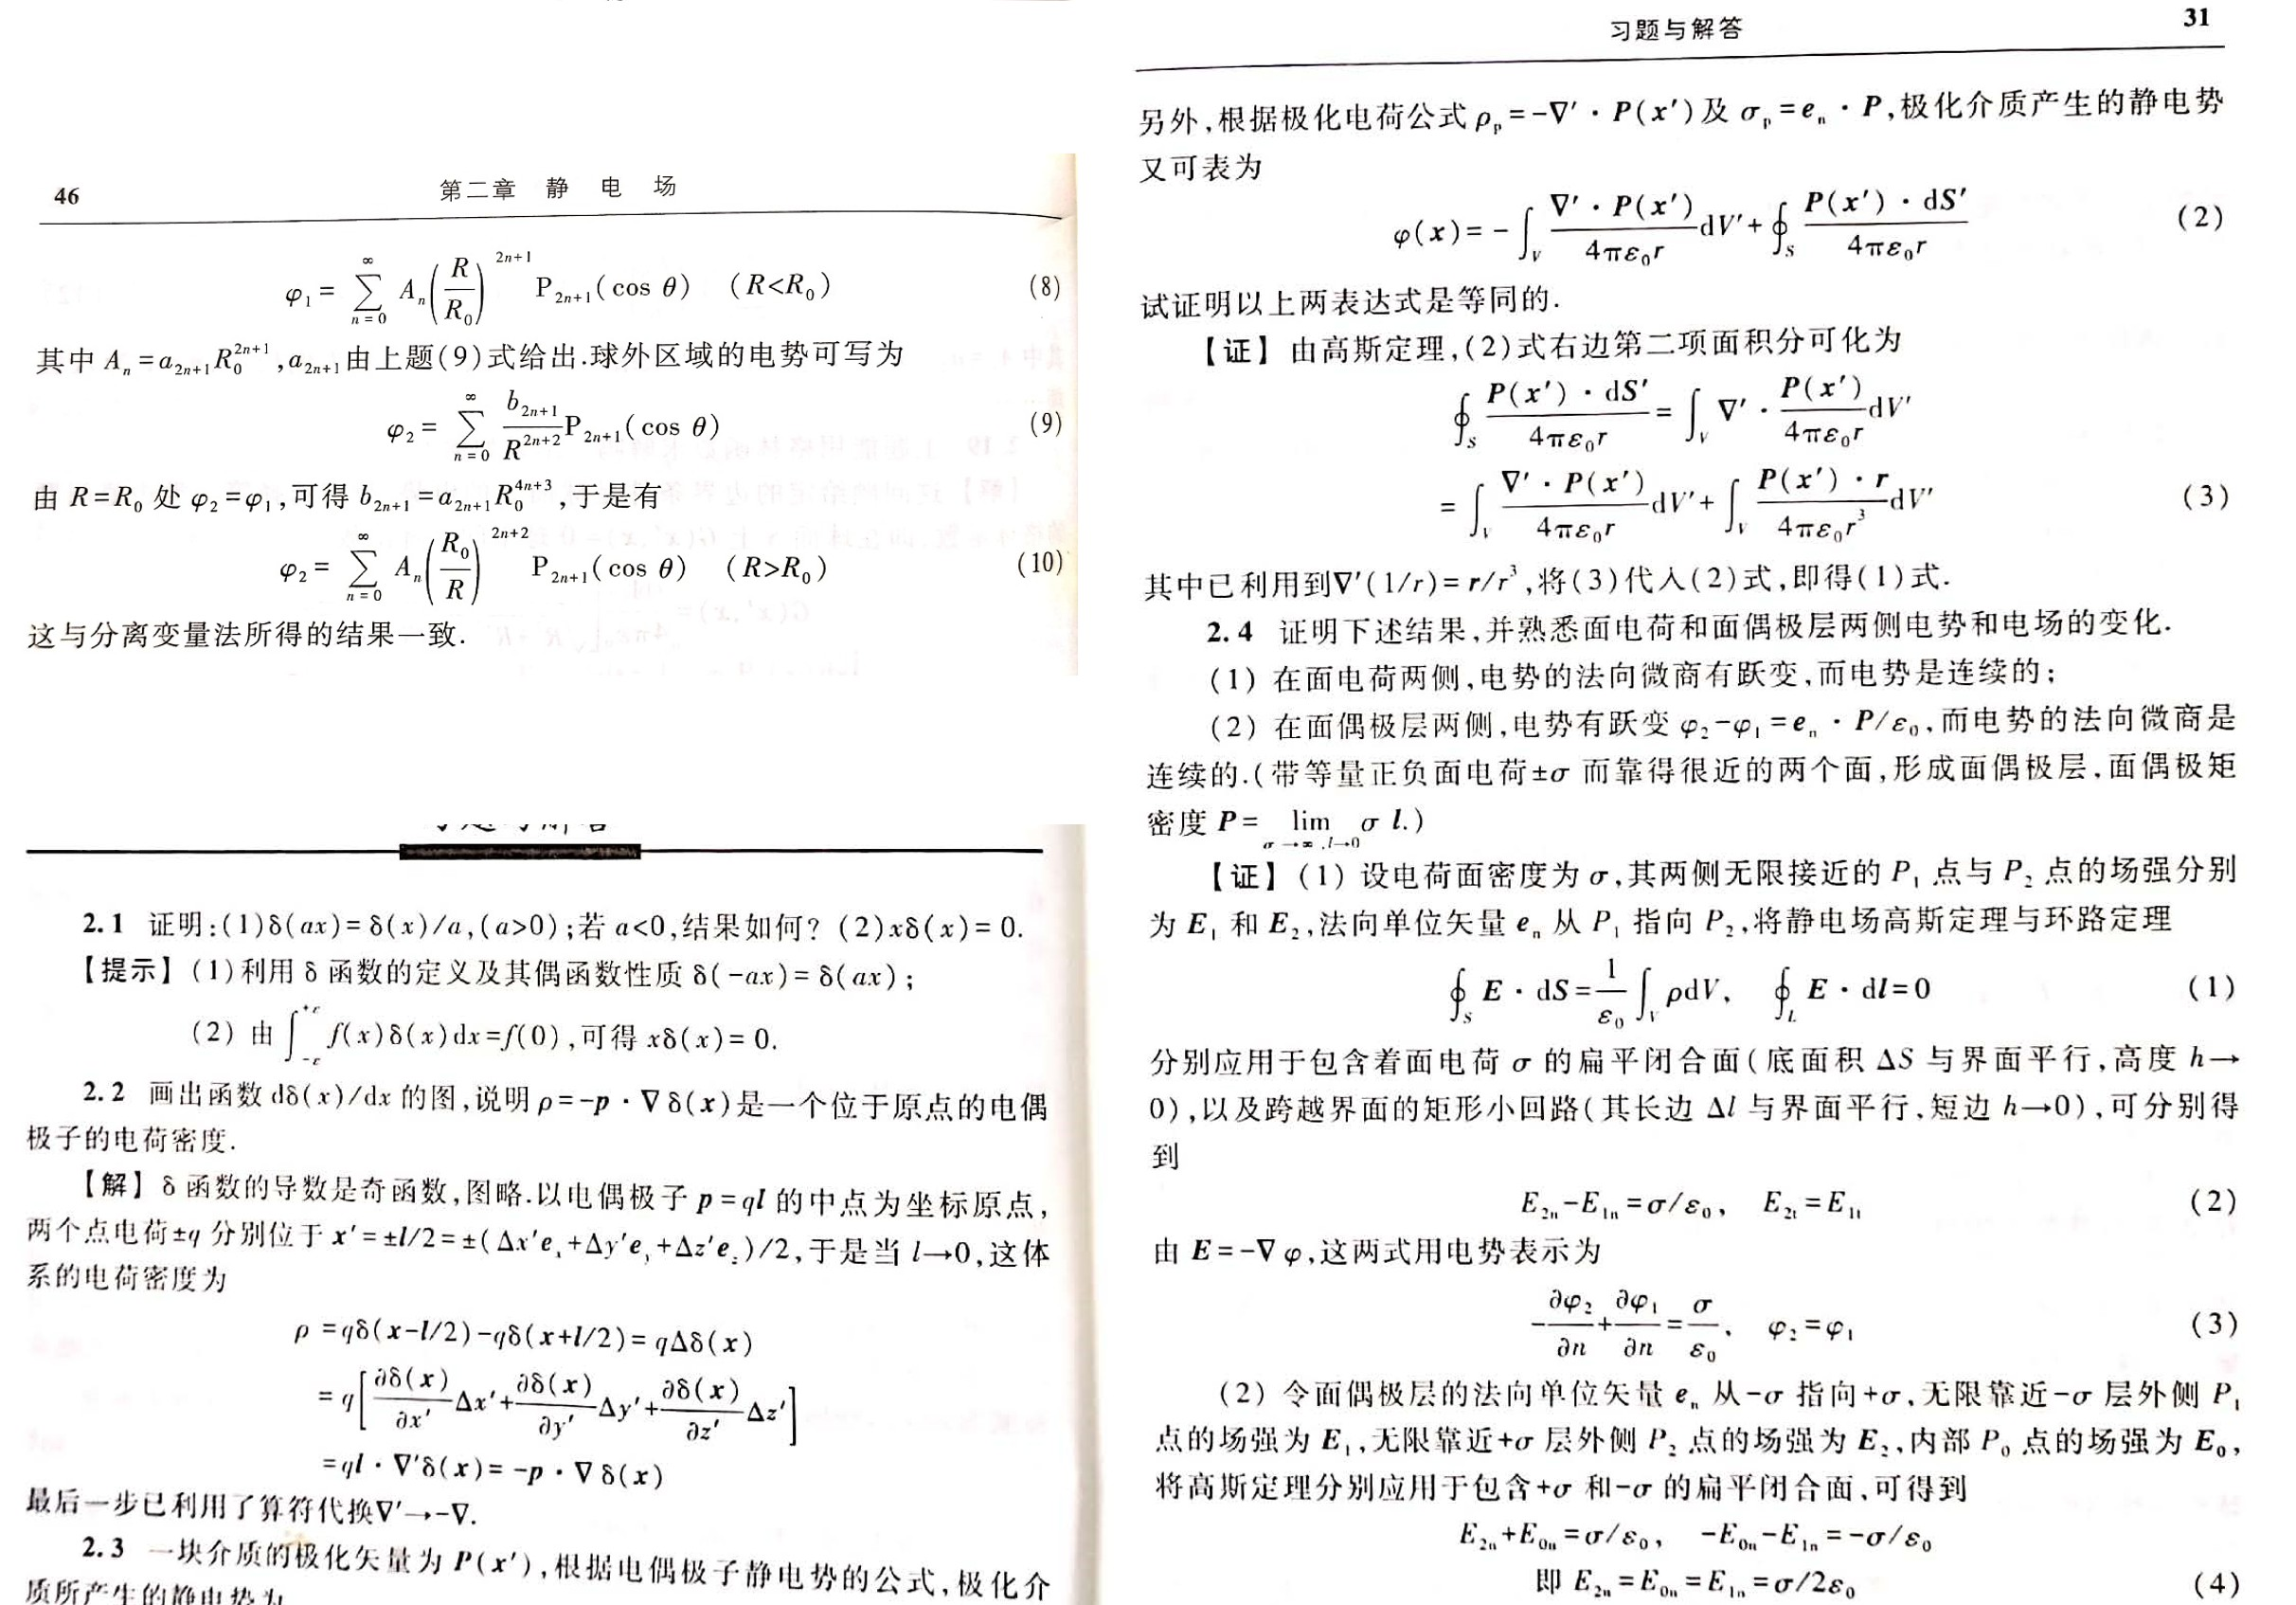
\includegraphics[scale=0.204]{1.jpg}}
    \end{minipage}
    \begin{minipage}[t]{0.48\textwidth}
        \centering
        \boxed{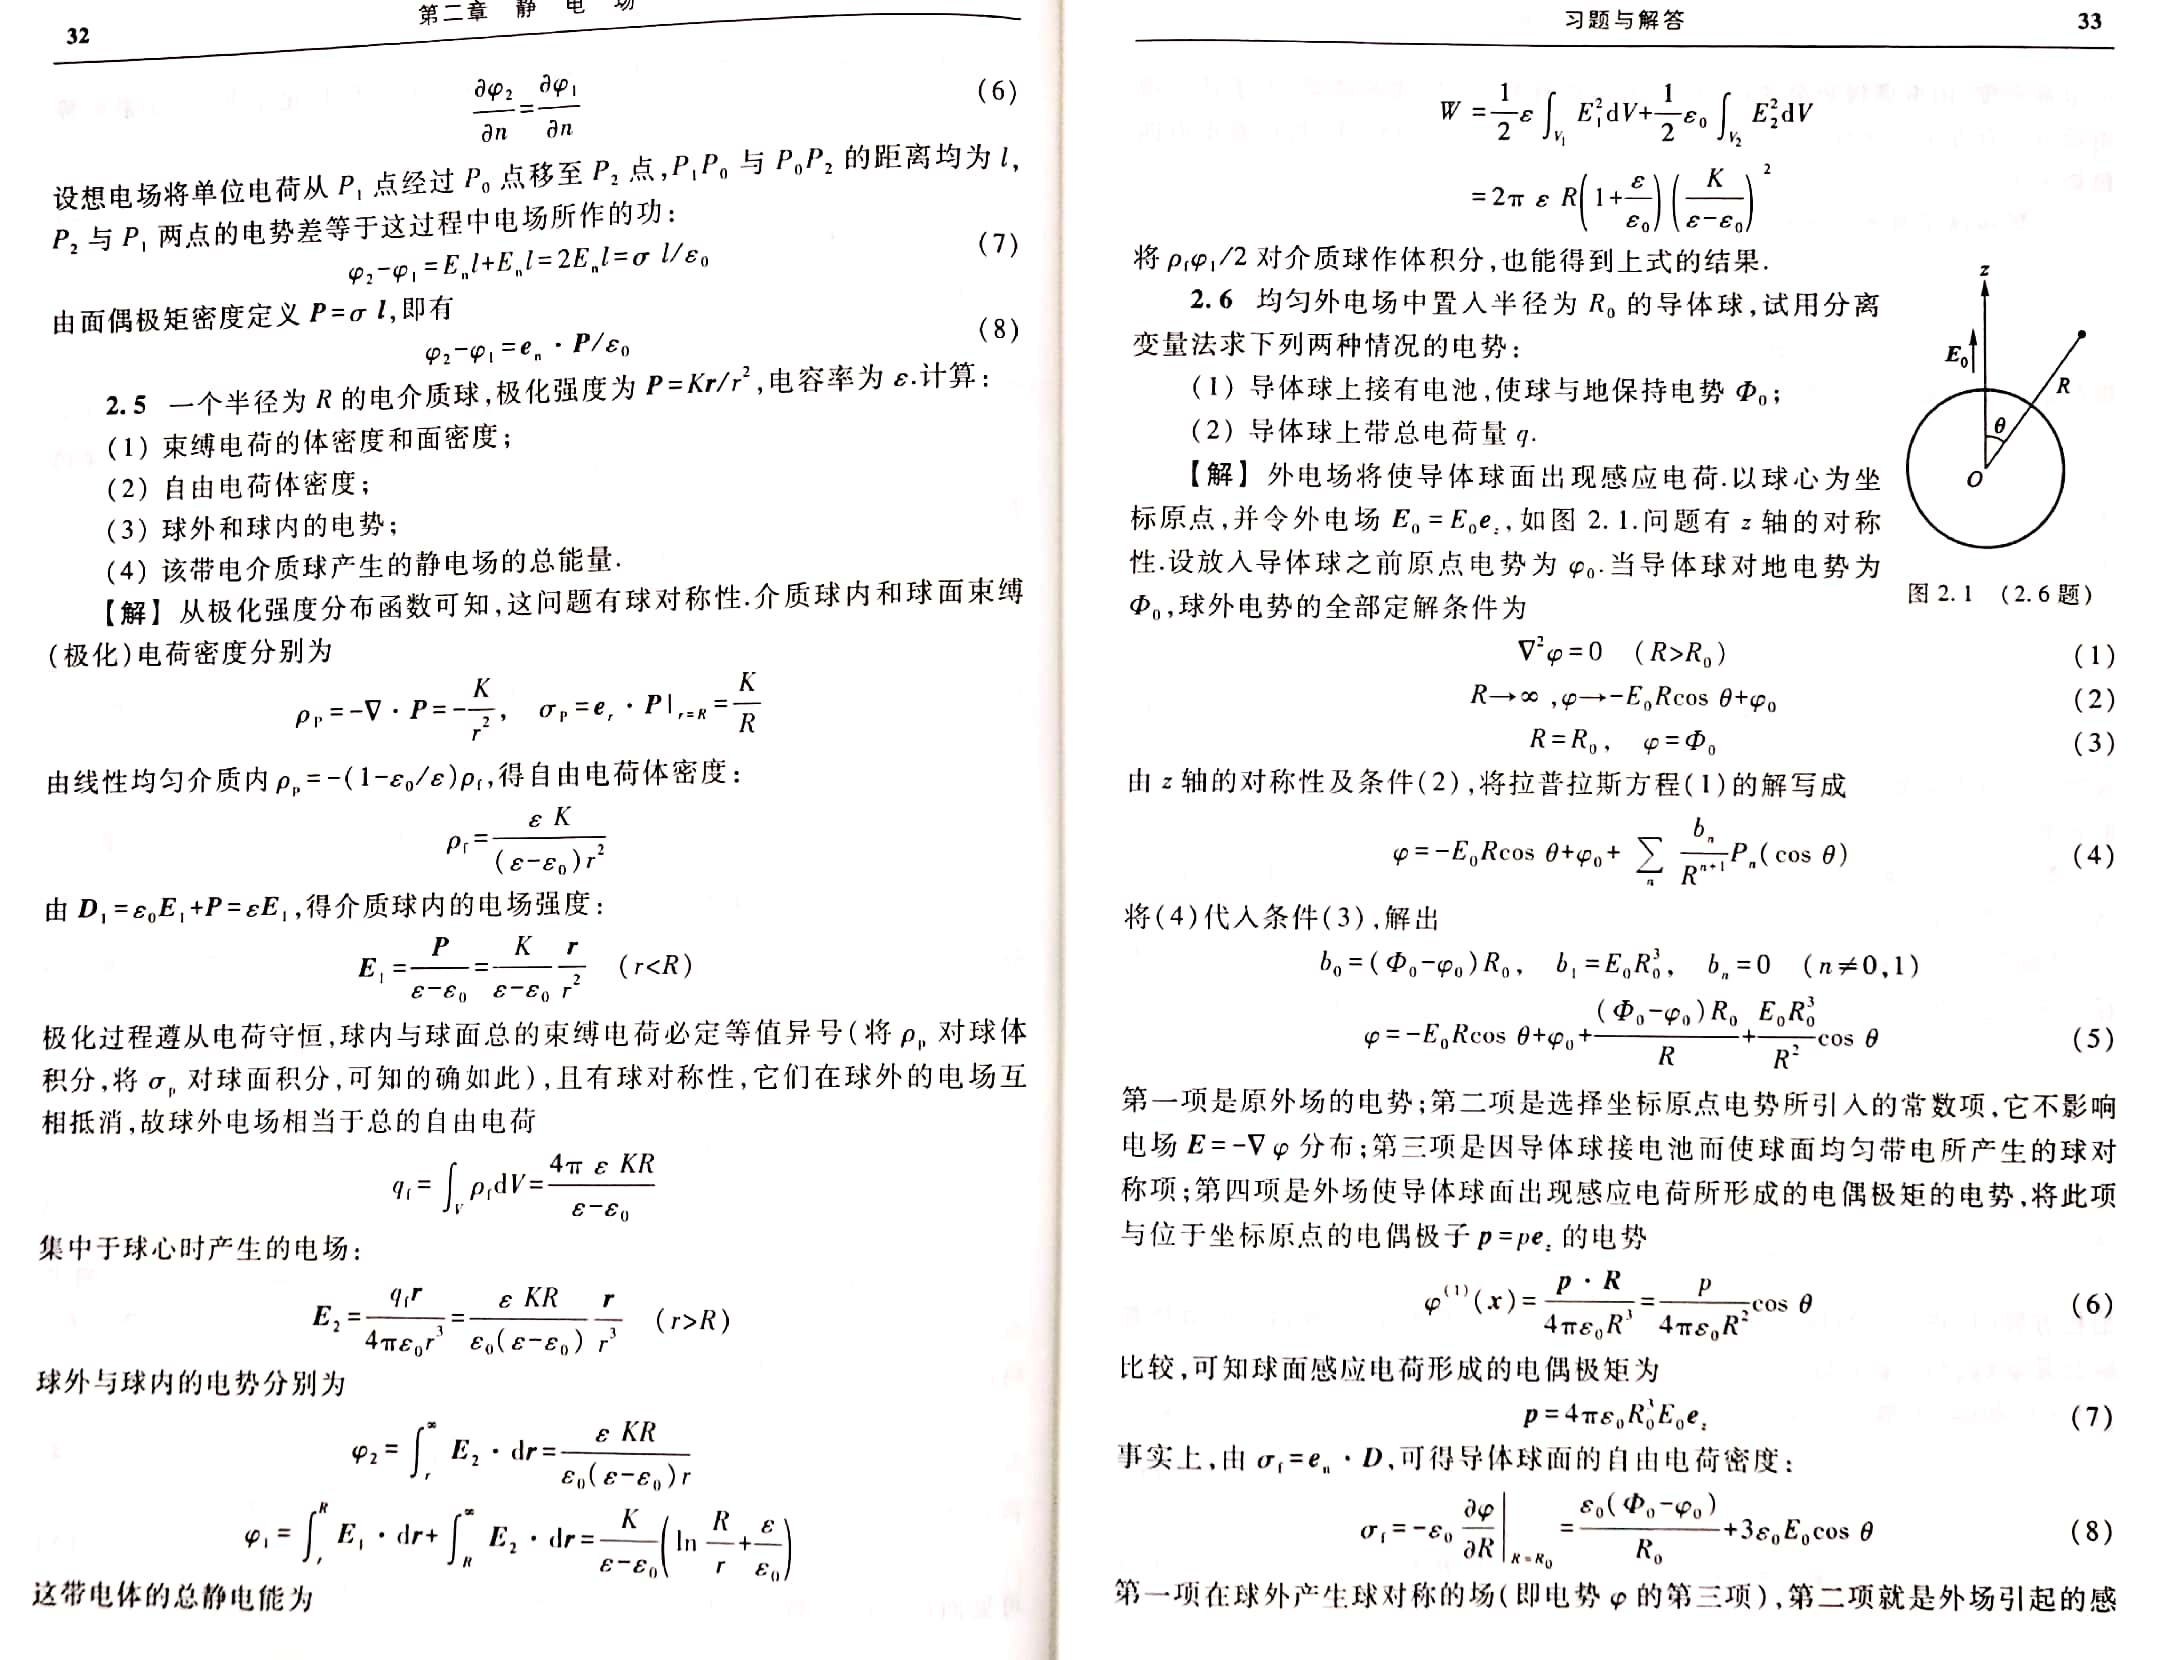
\includegraphics[scale=0.47]{2.jpg}}
    \end{minipage}
\end{figure}
\begin{figure}[htbp]
    \centering
    \begin{minipage}[t]{0.5\textwidth}
        \centering
        \boxed{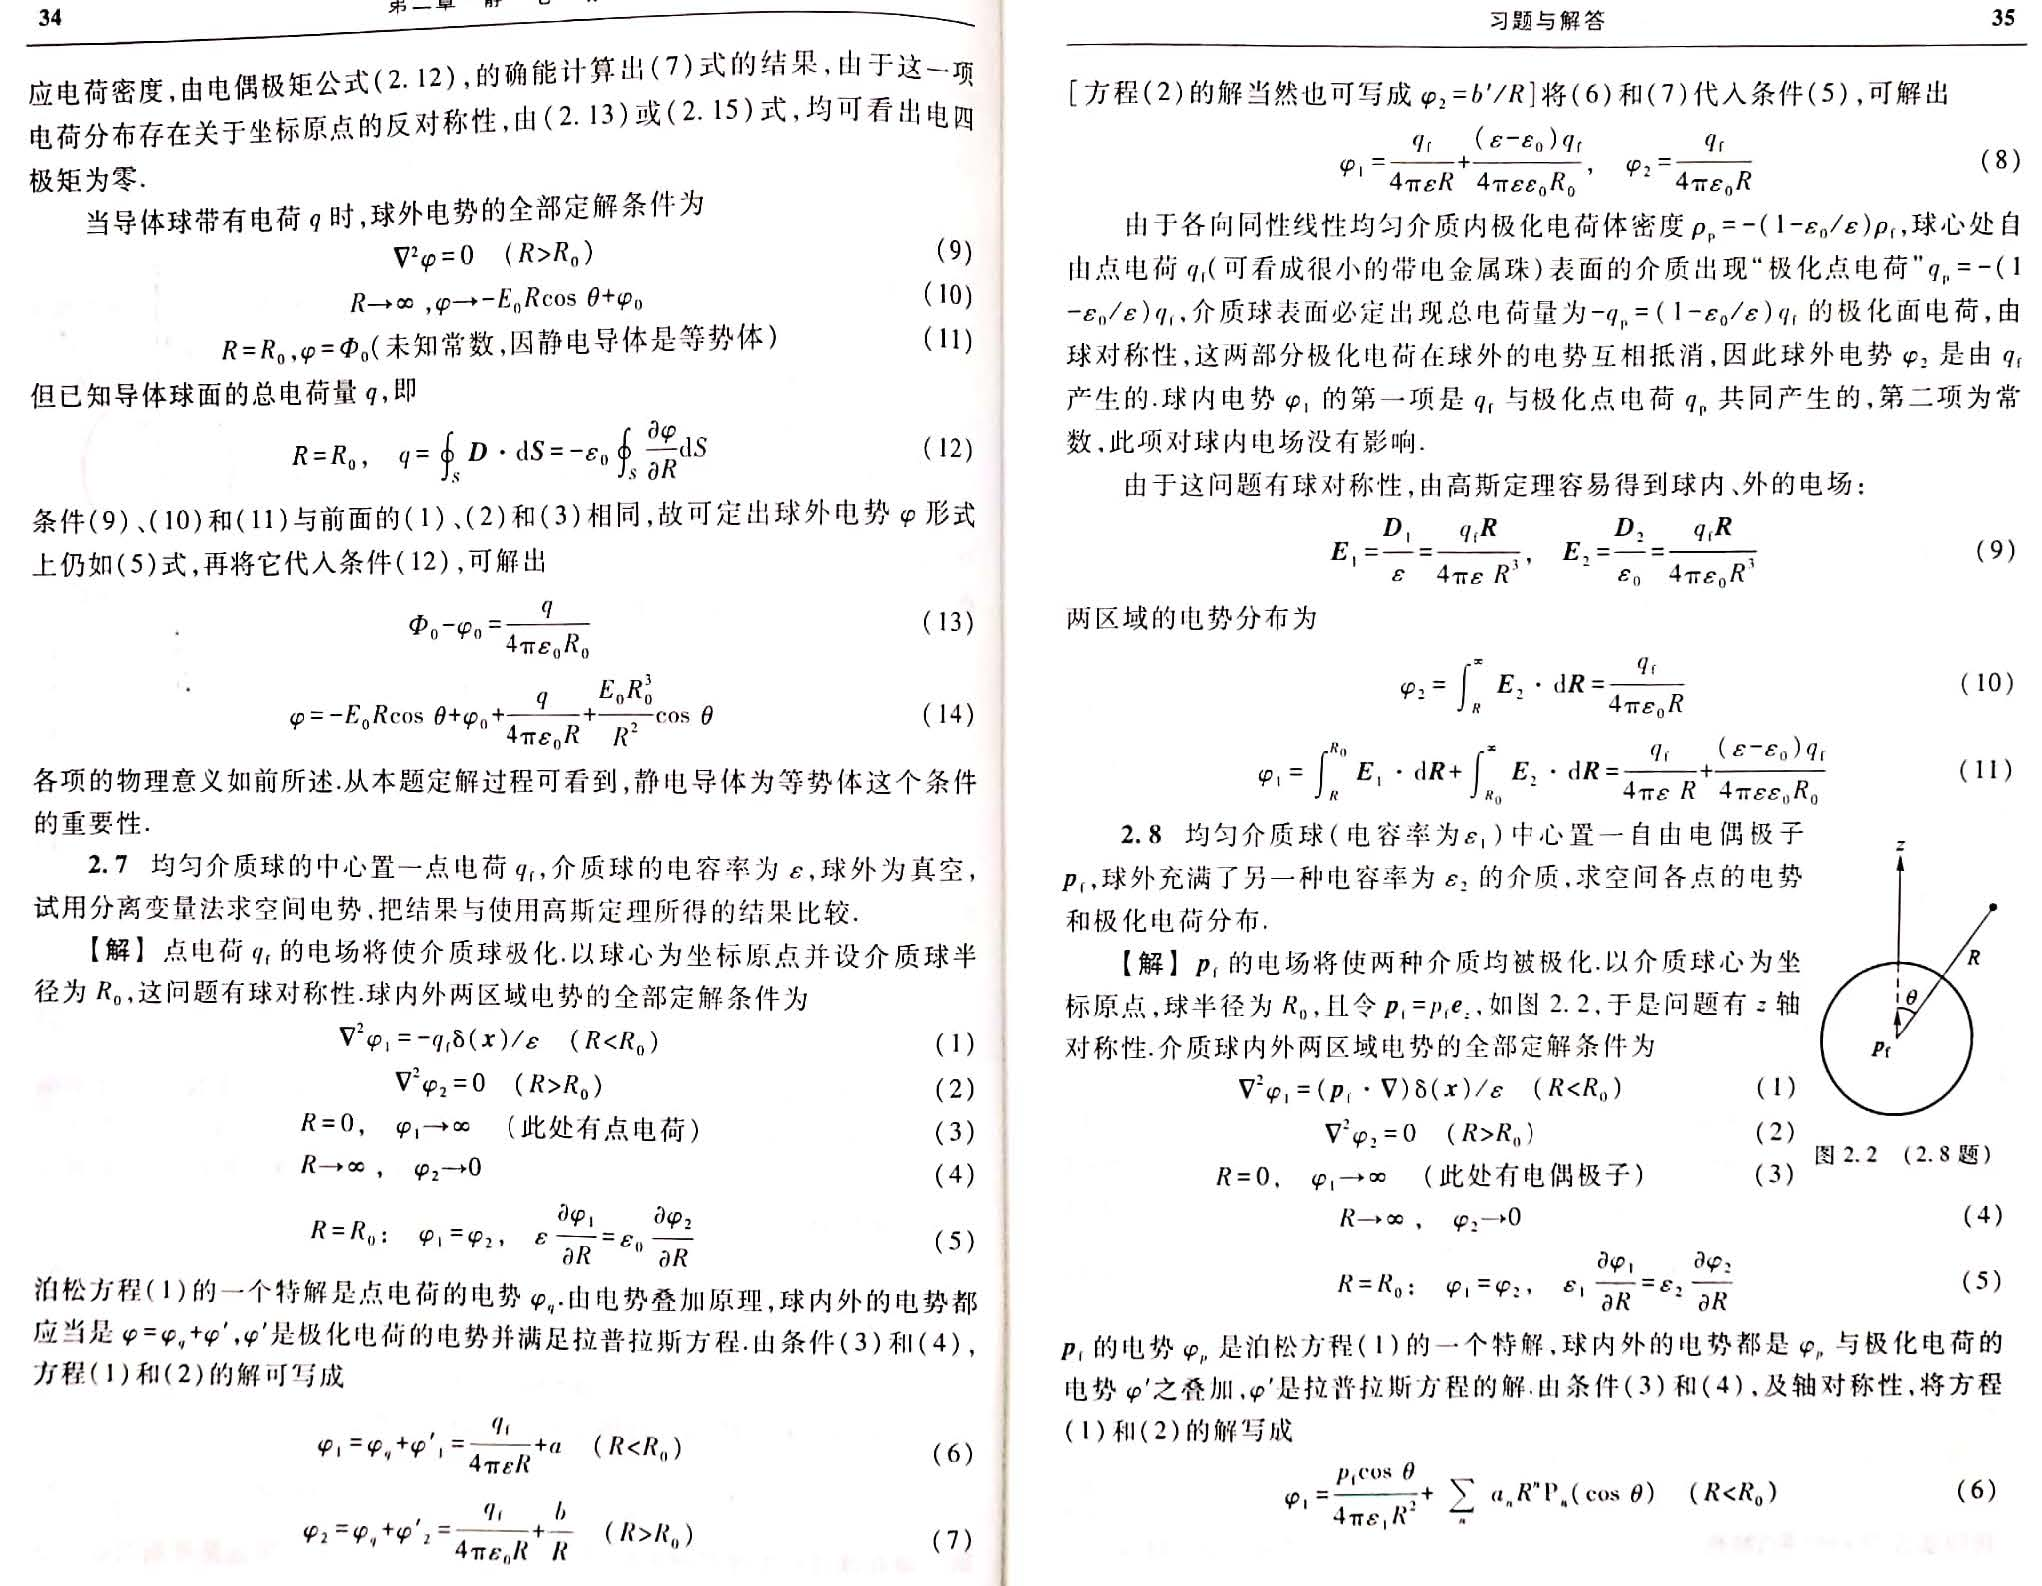
\includegraphics[scale=0.5]{3.jpg}}
    \end{minipage}
    \begin{minipage}[t]{0.48\textwidth}
        \centering
        \boxed{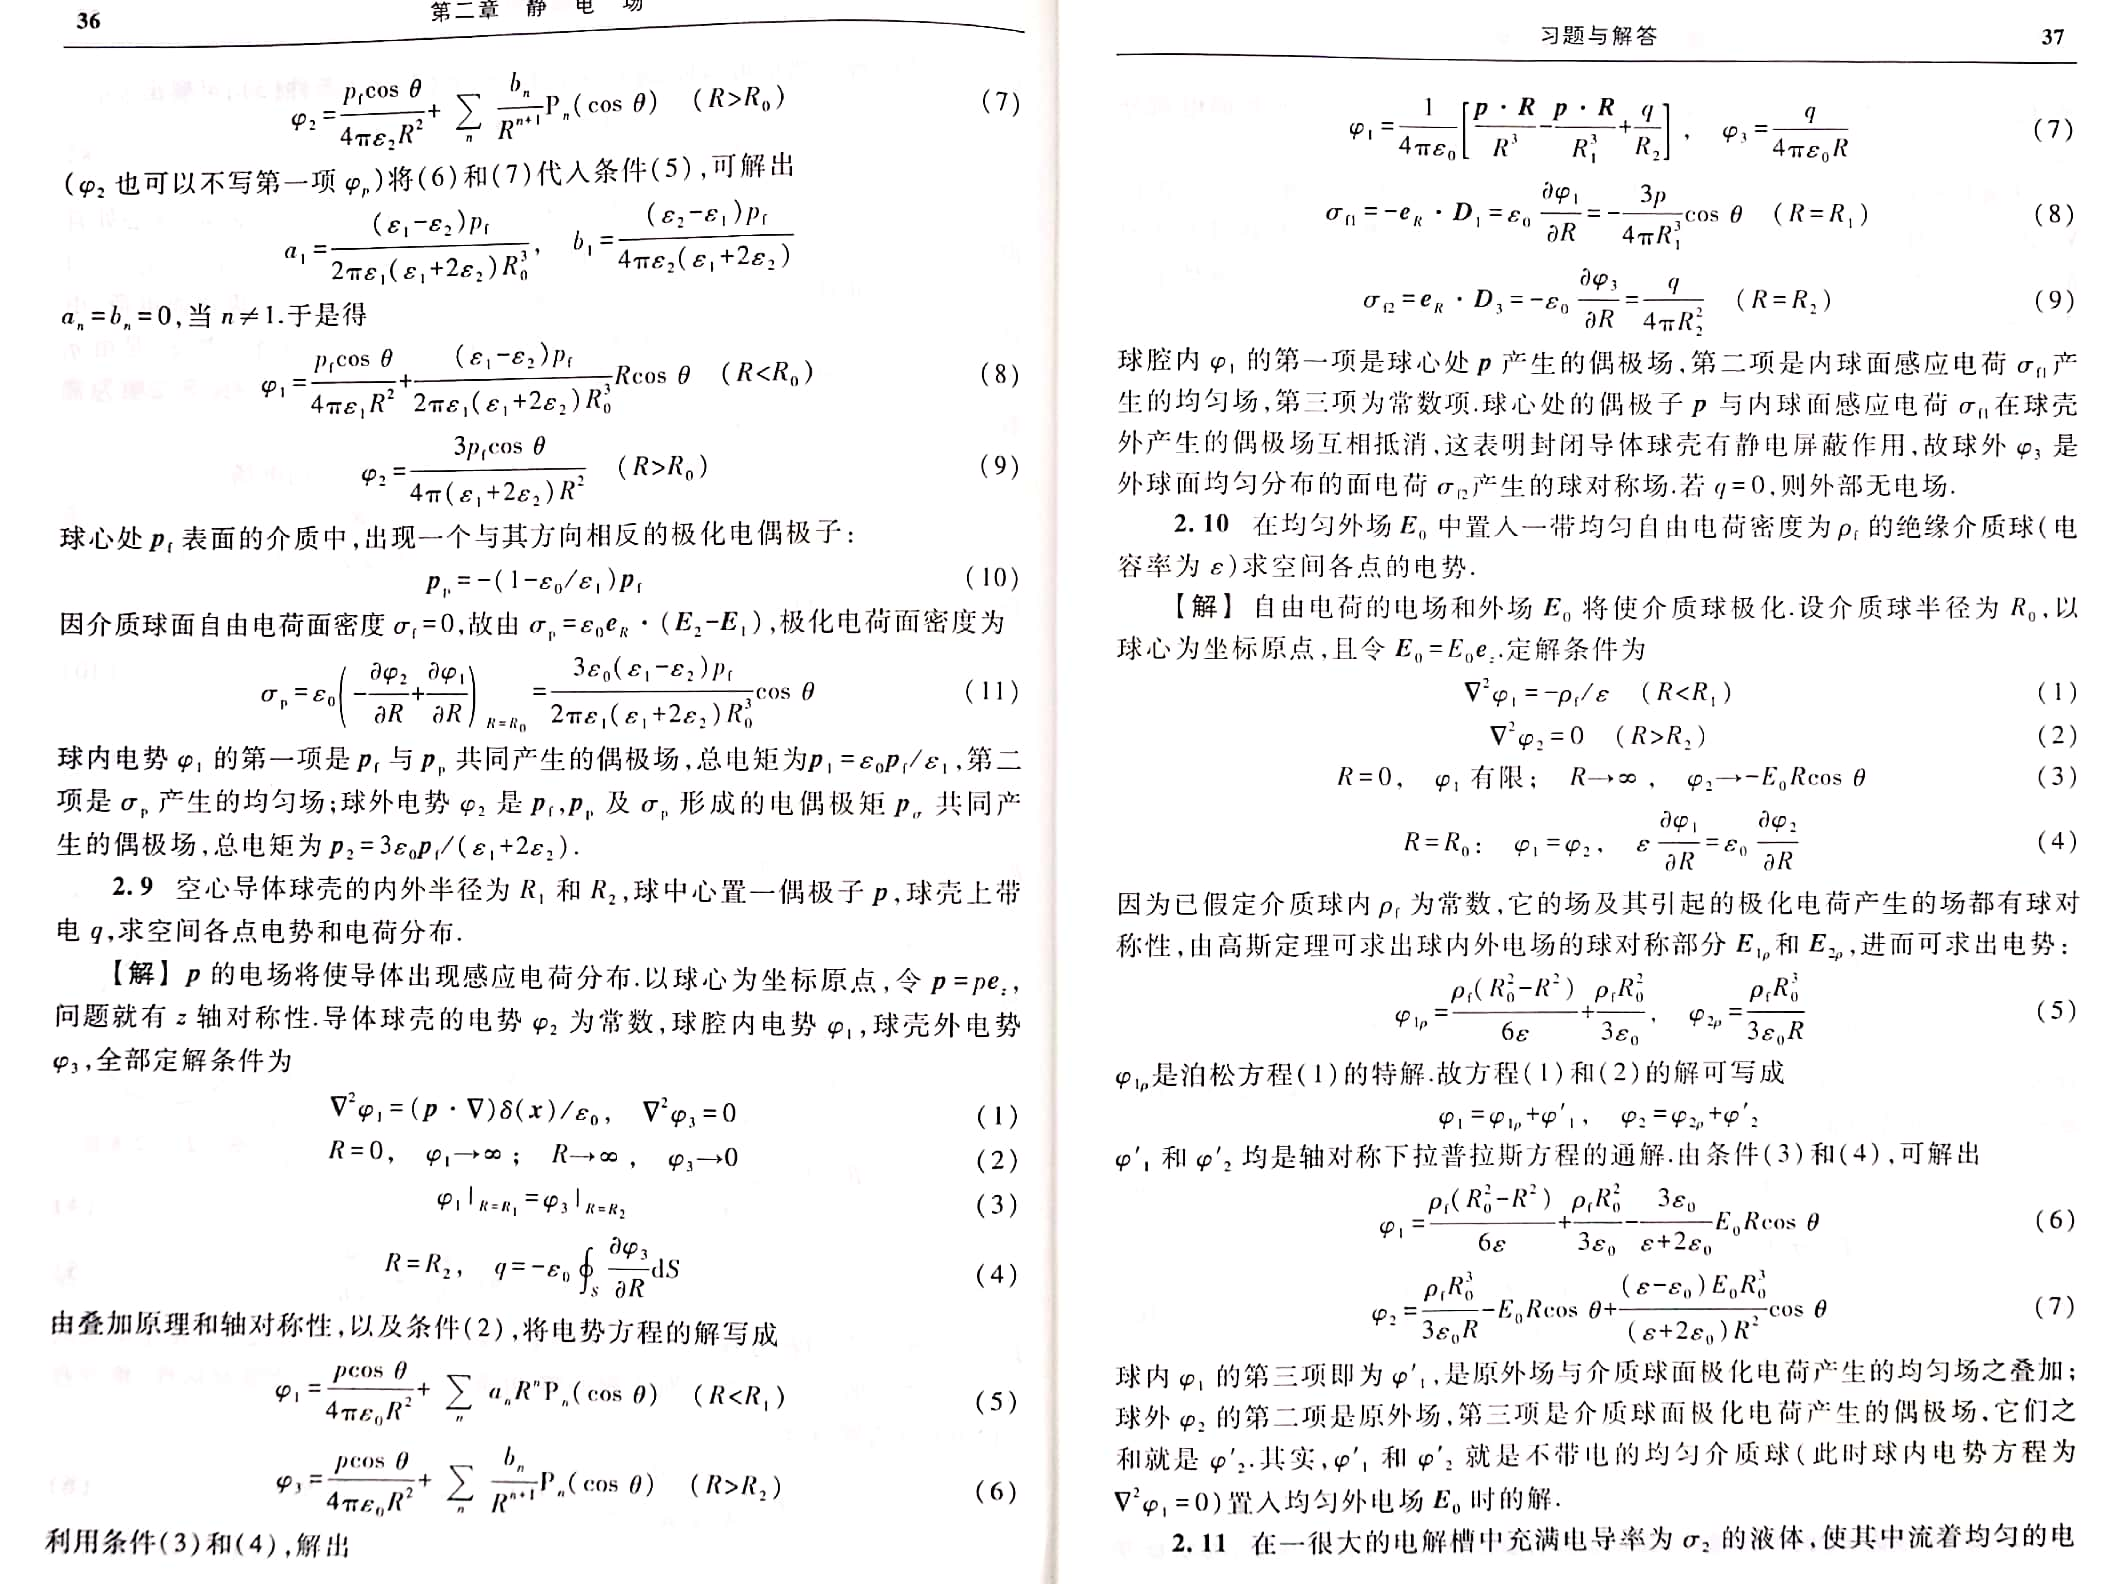
\includegraphics[scale=0.5]{4.jpg}}
    \end{minipage}
    \begin{minipage}[t]{0.5\textwidth}
        \centering
        \boxed{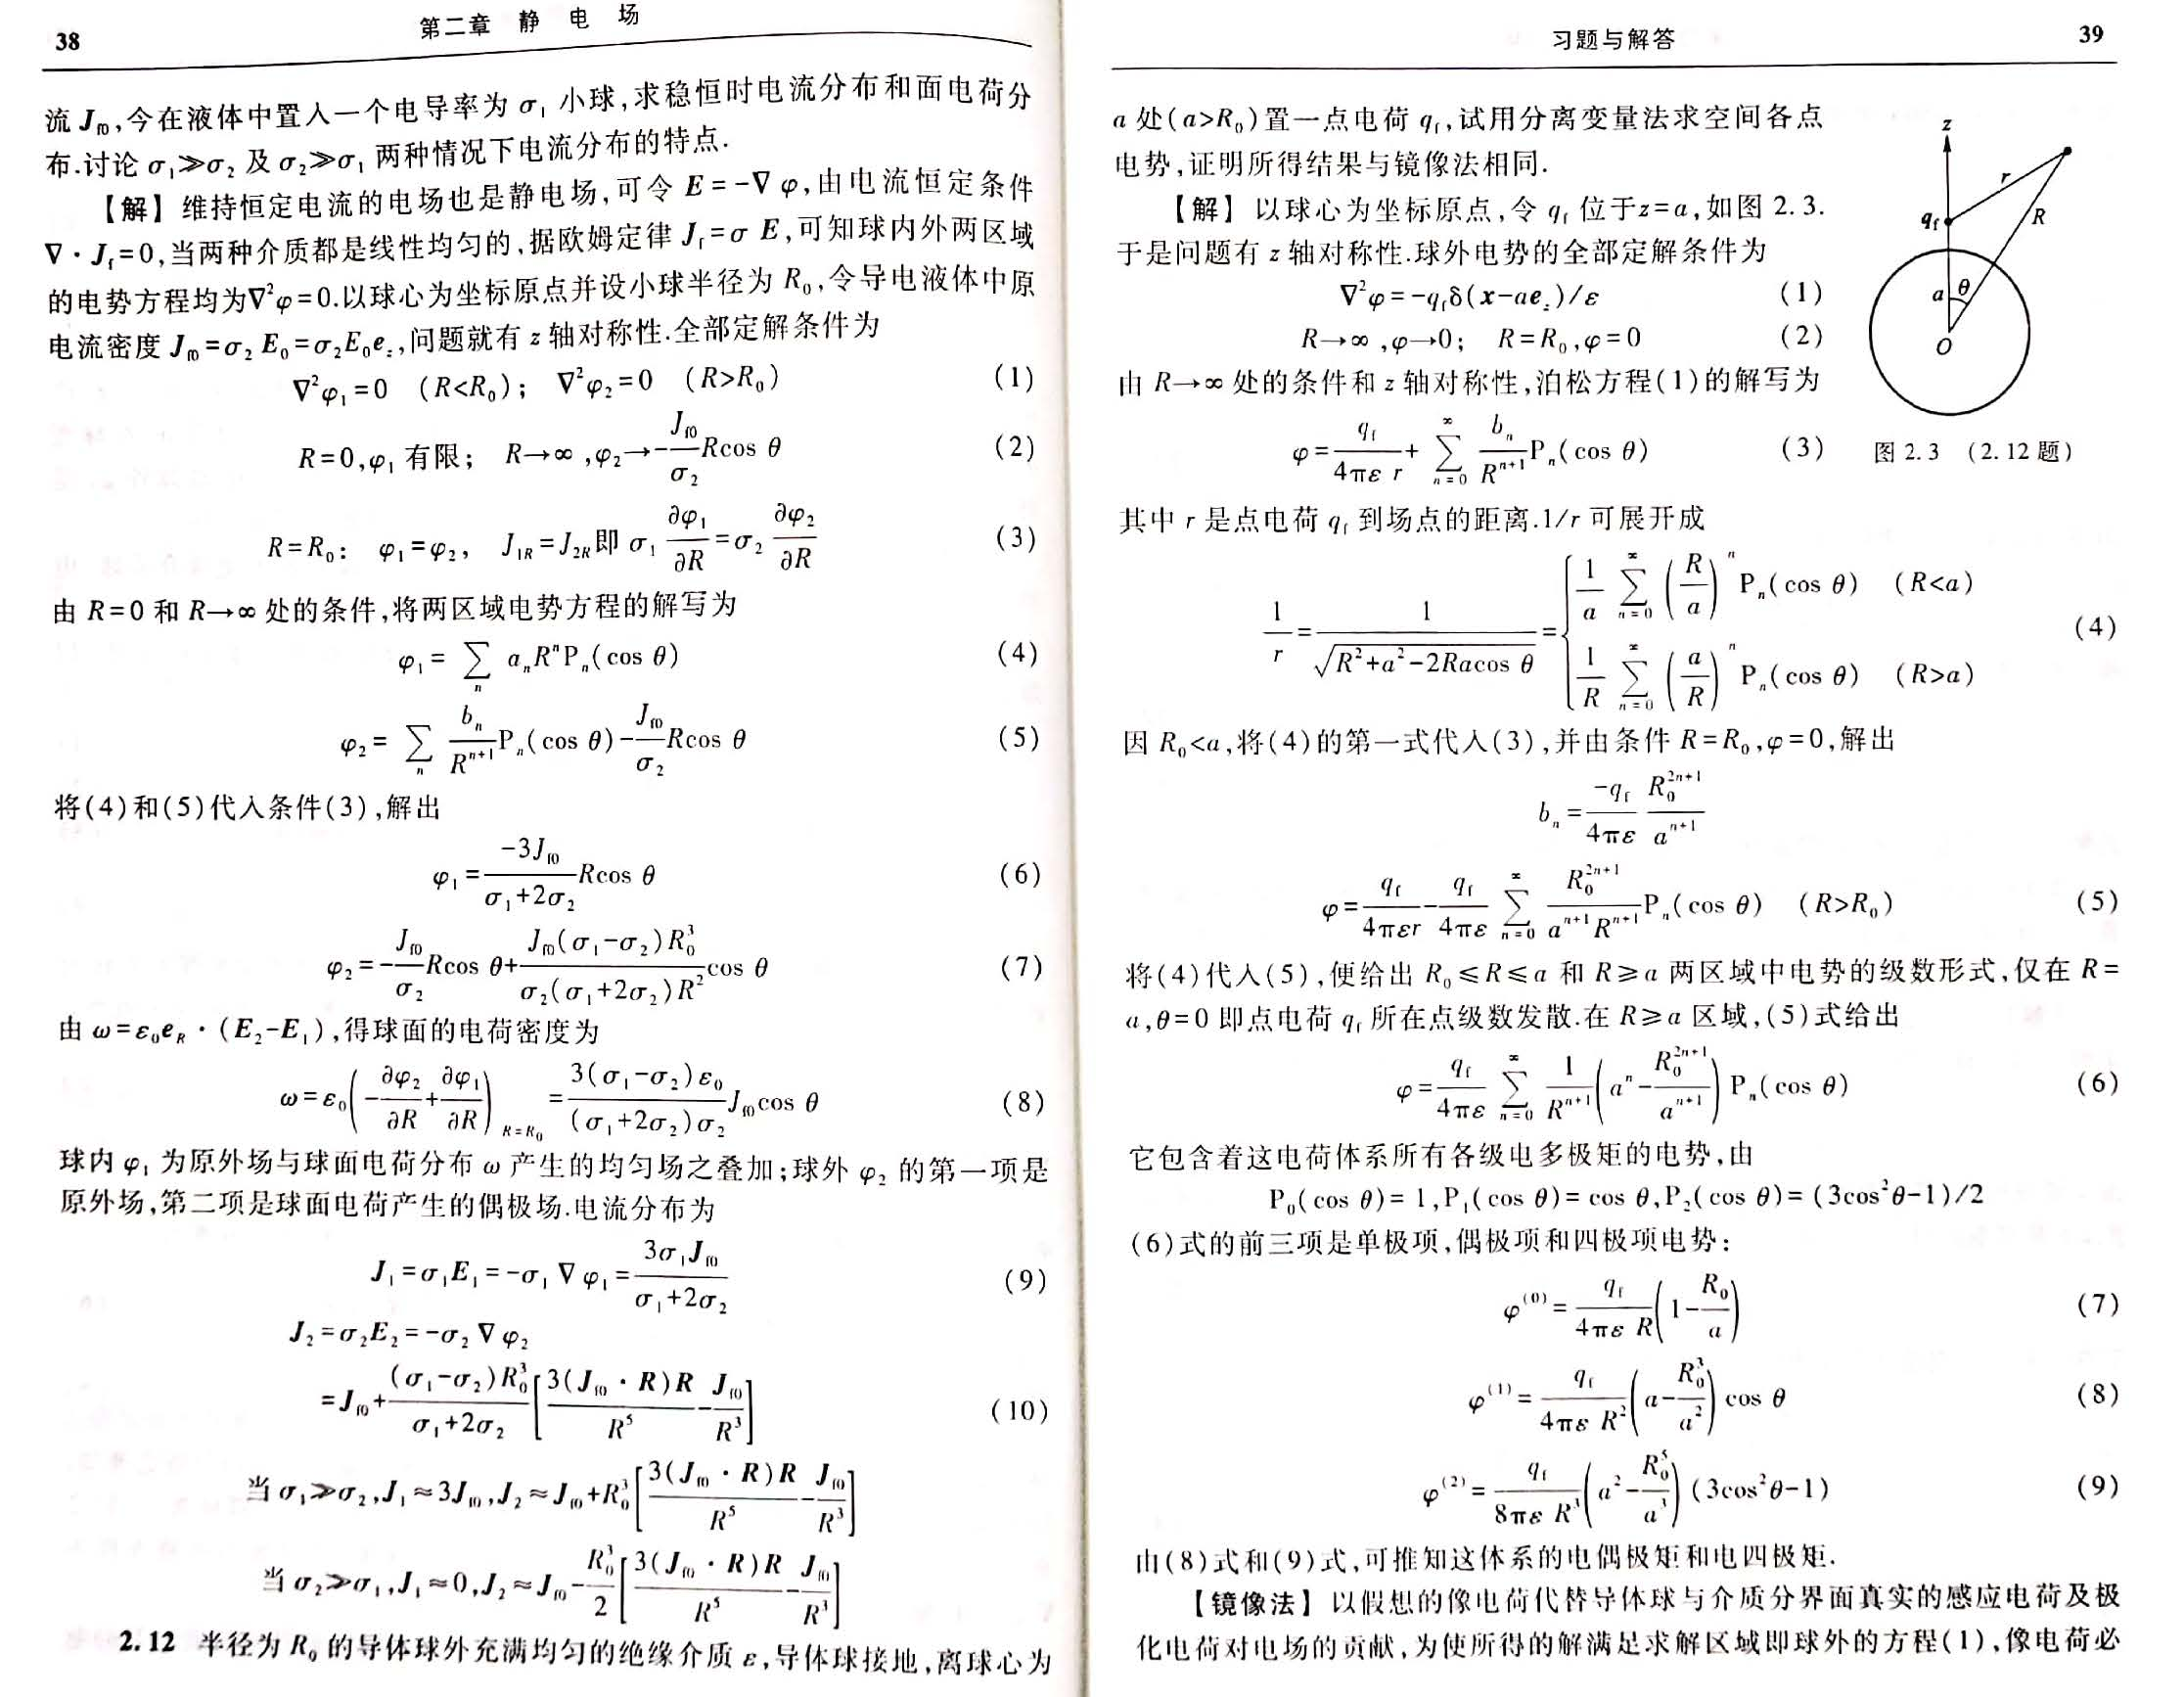
\includegraphics[scale=0.5]{5.jpg}}
    \end{minipage}
    \begin{minipage}[t]{0.48\textwidth}
        \centering
        \boxed{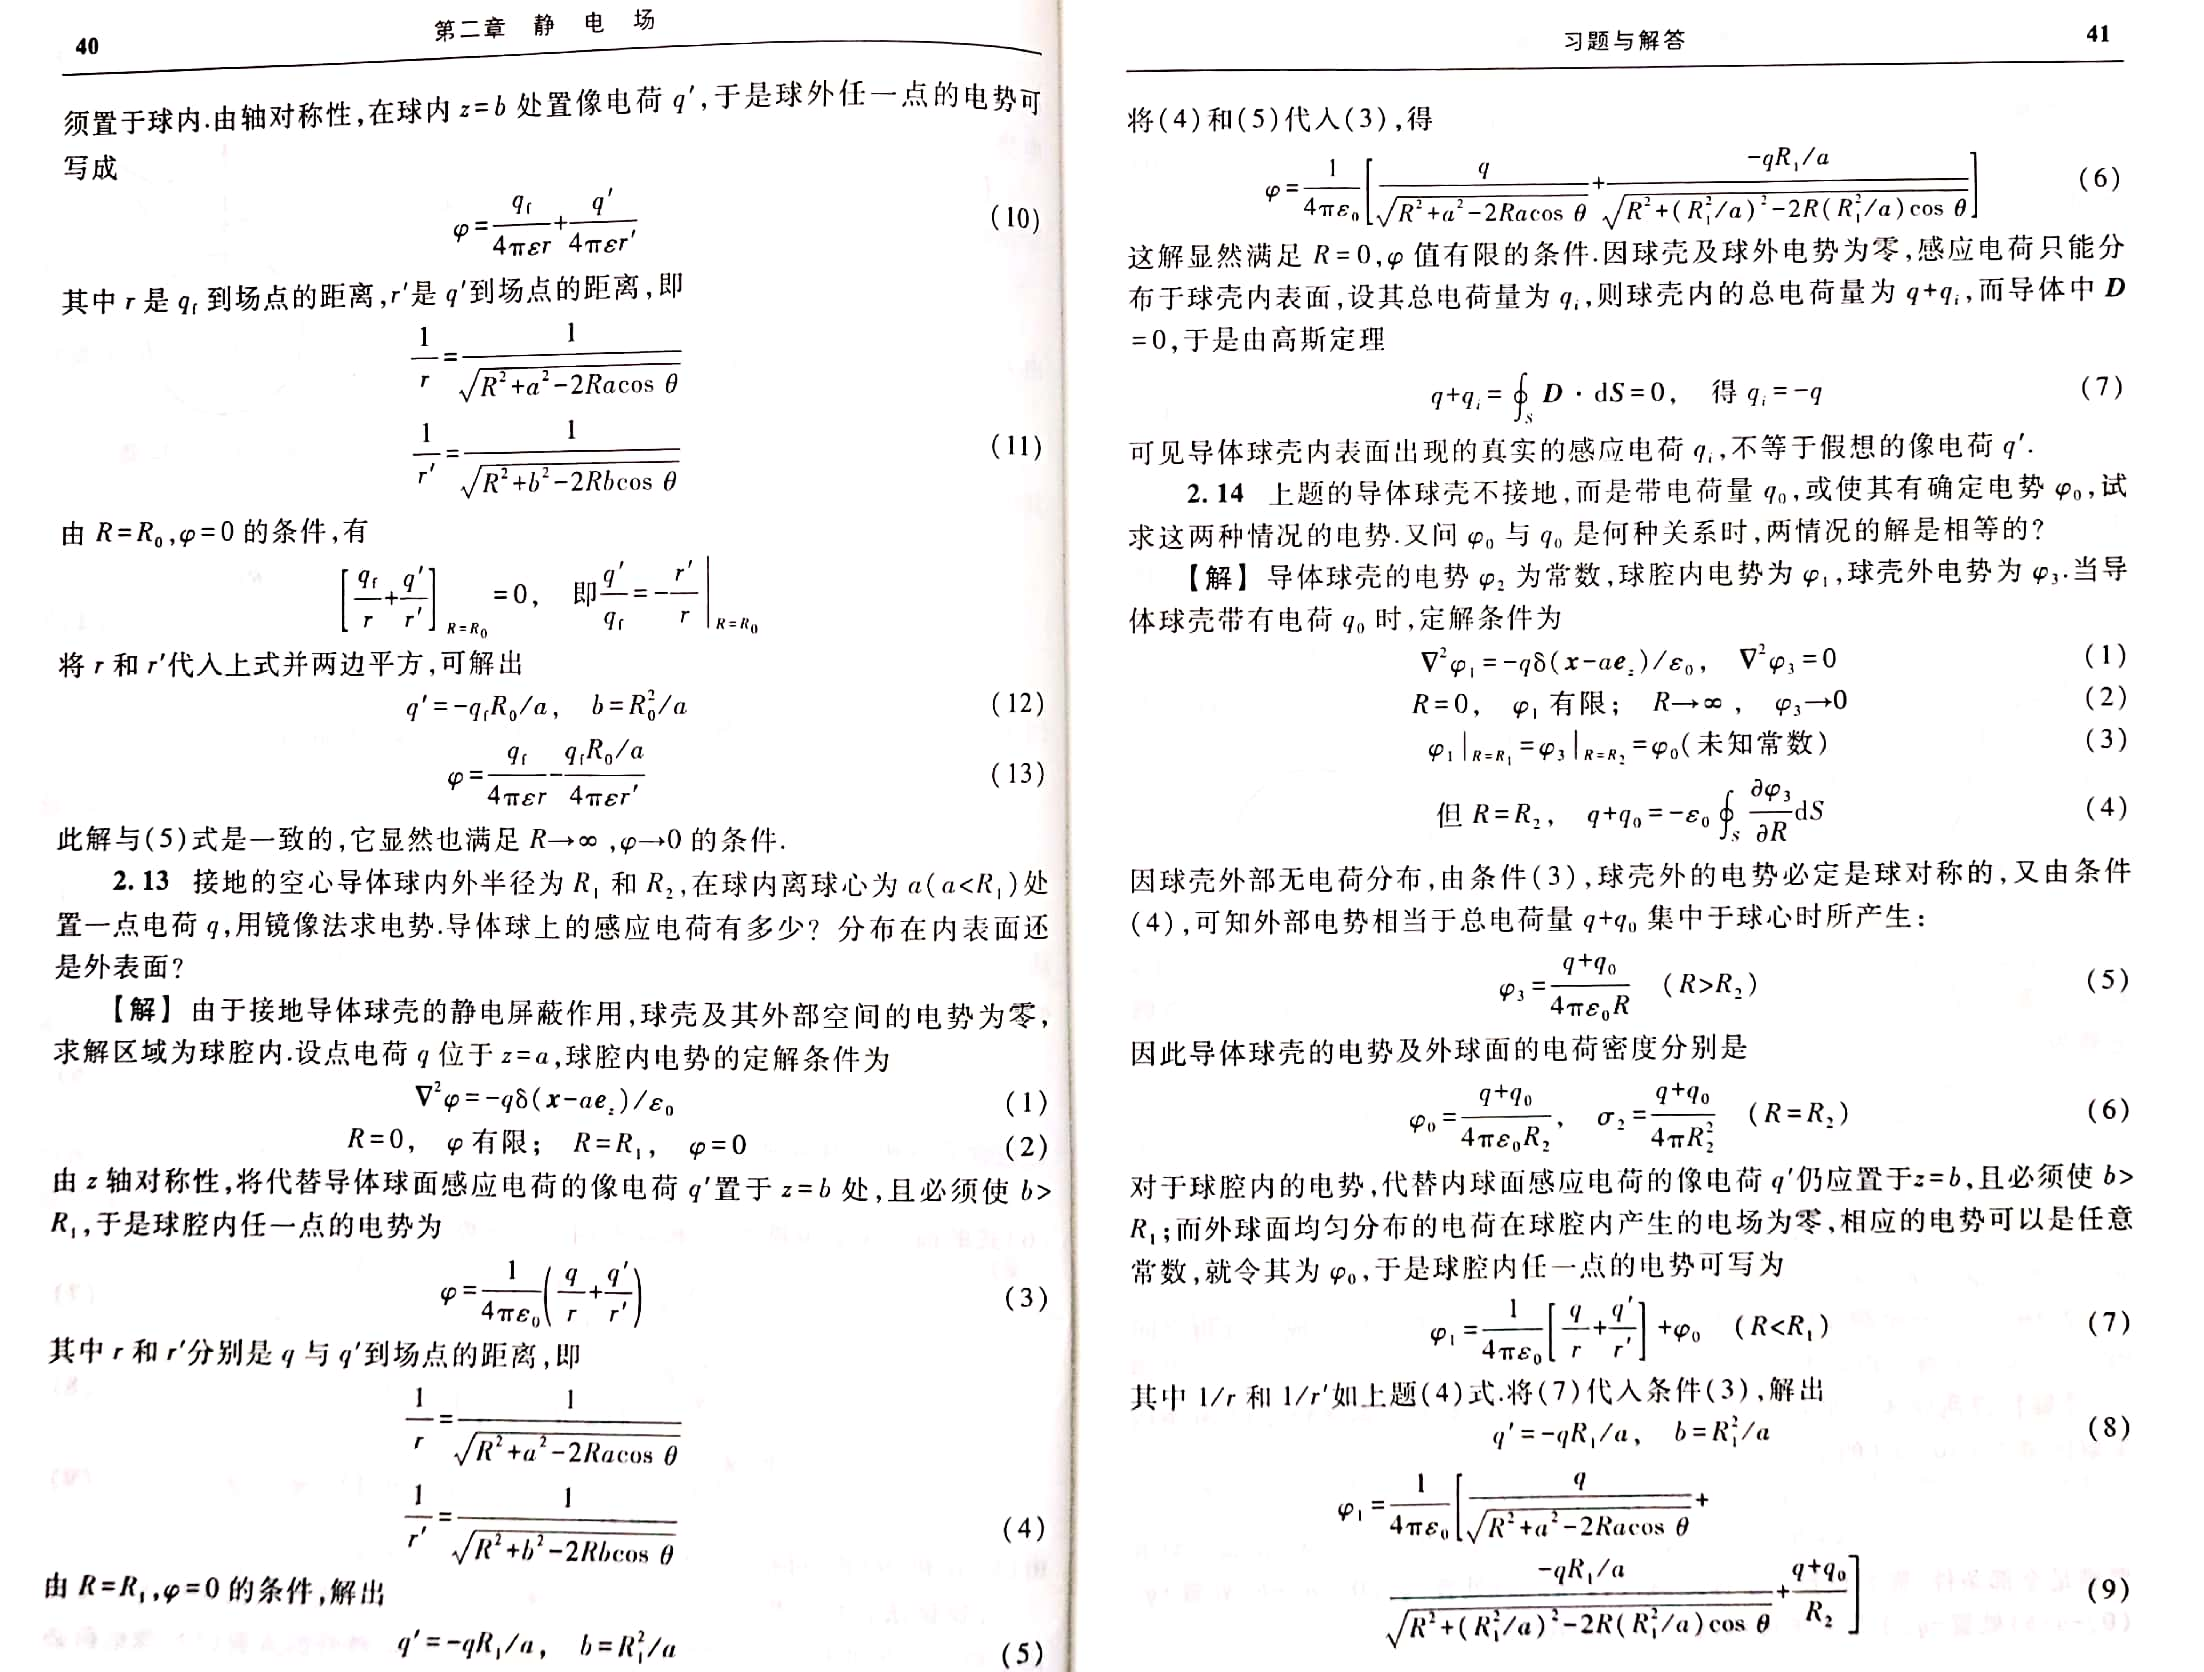
\includegraphics[scale=0.5]{6.jpg}}
    \end{minipage}
    \begin{minipage}[t]{0.5\textwidth}
        \centering
        \boxed{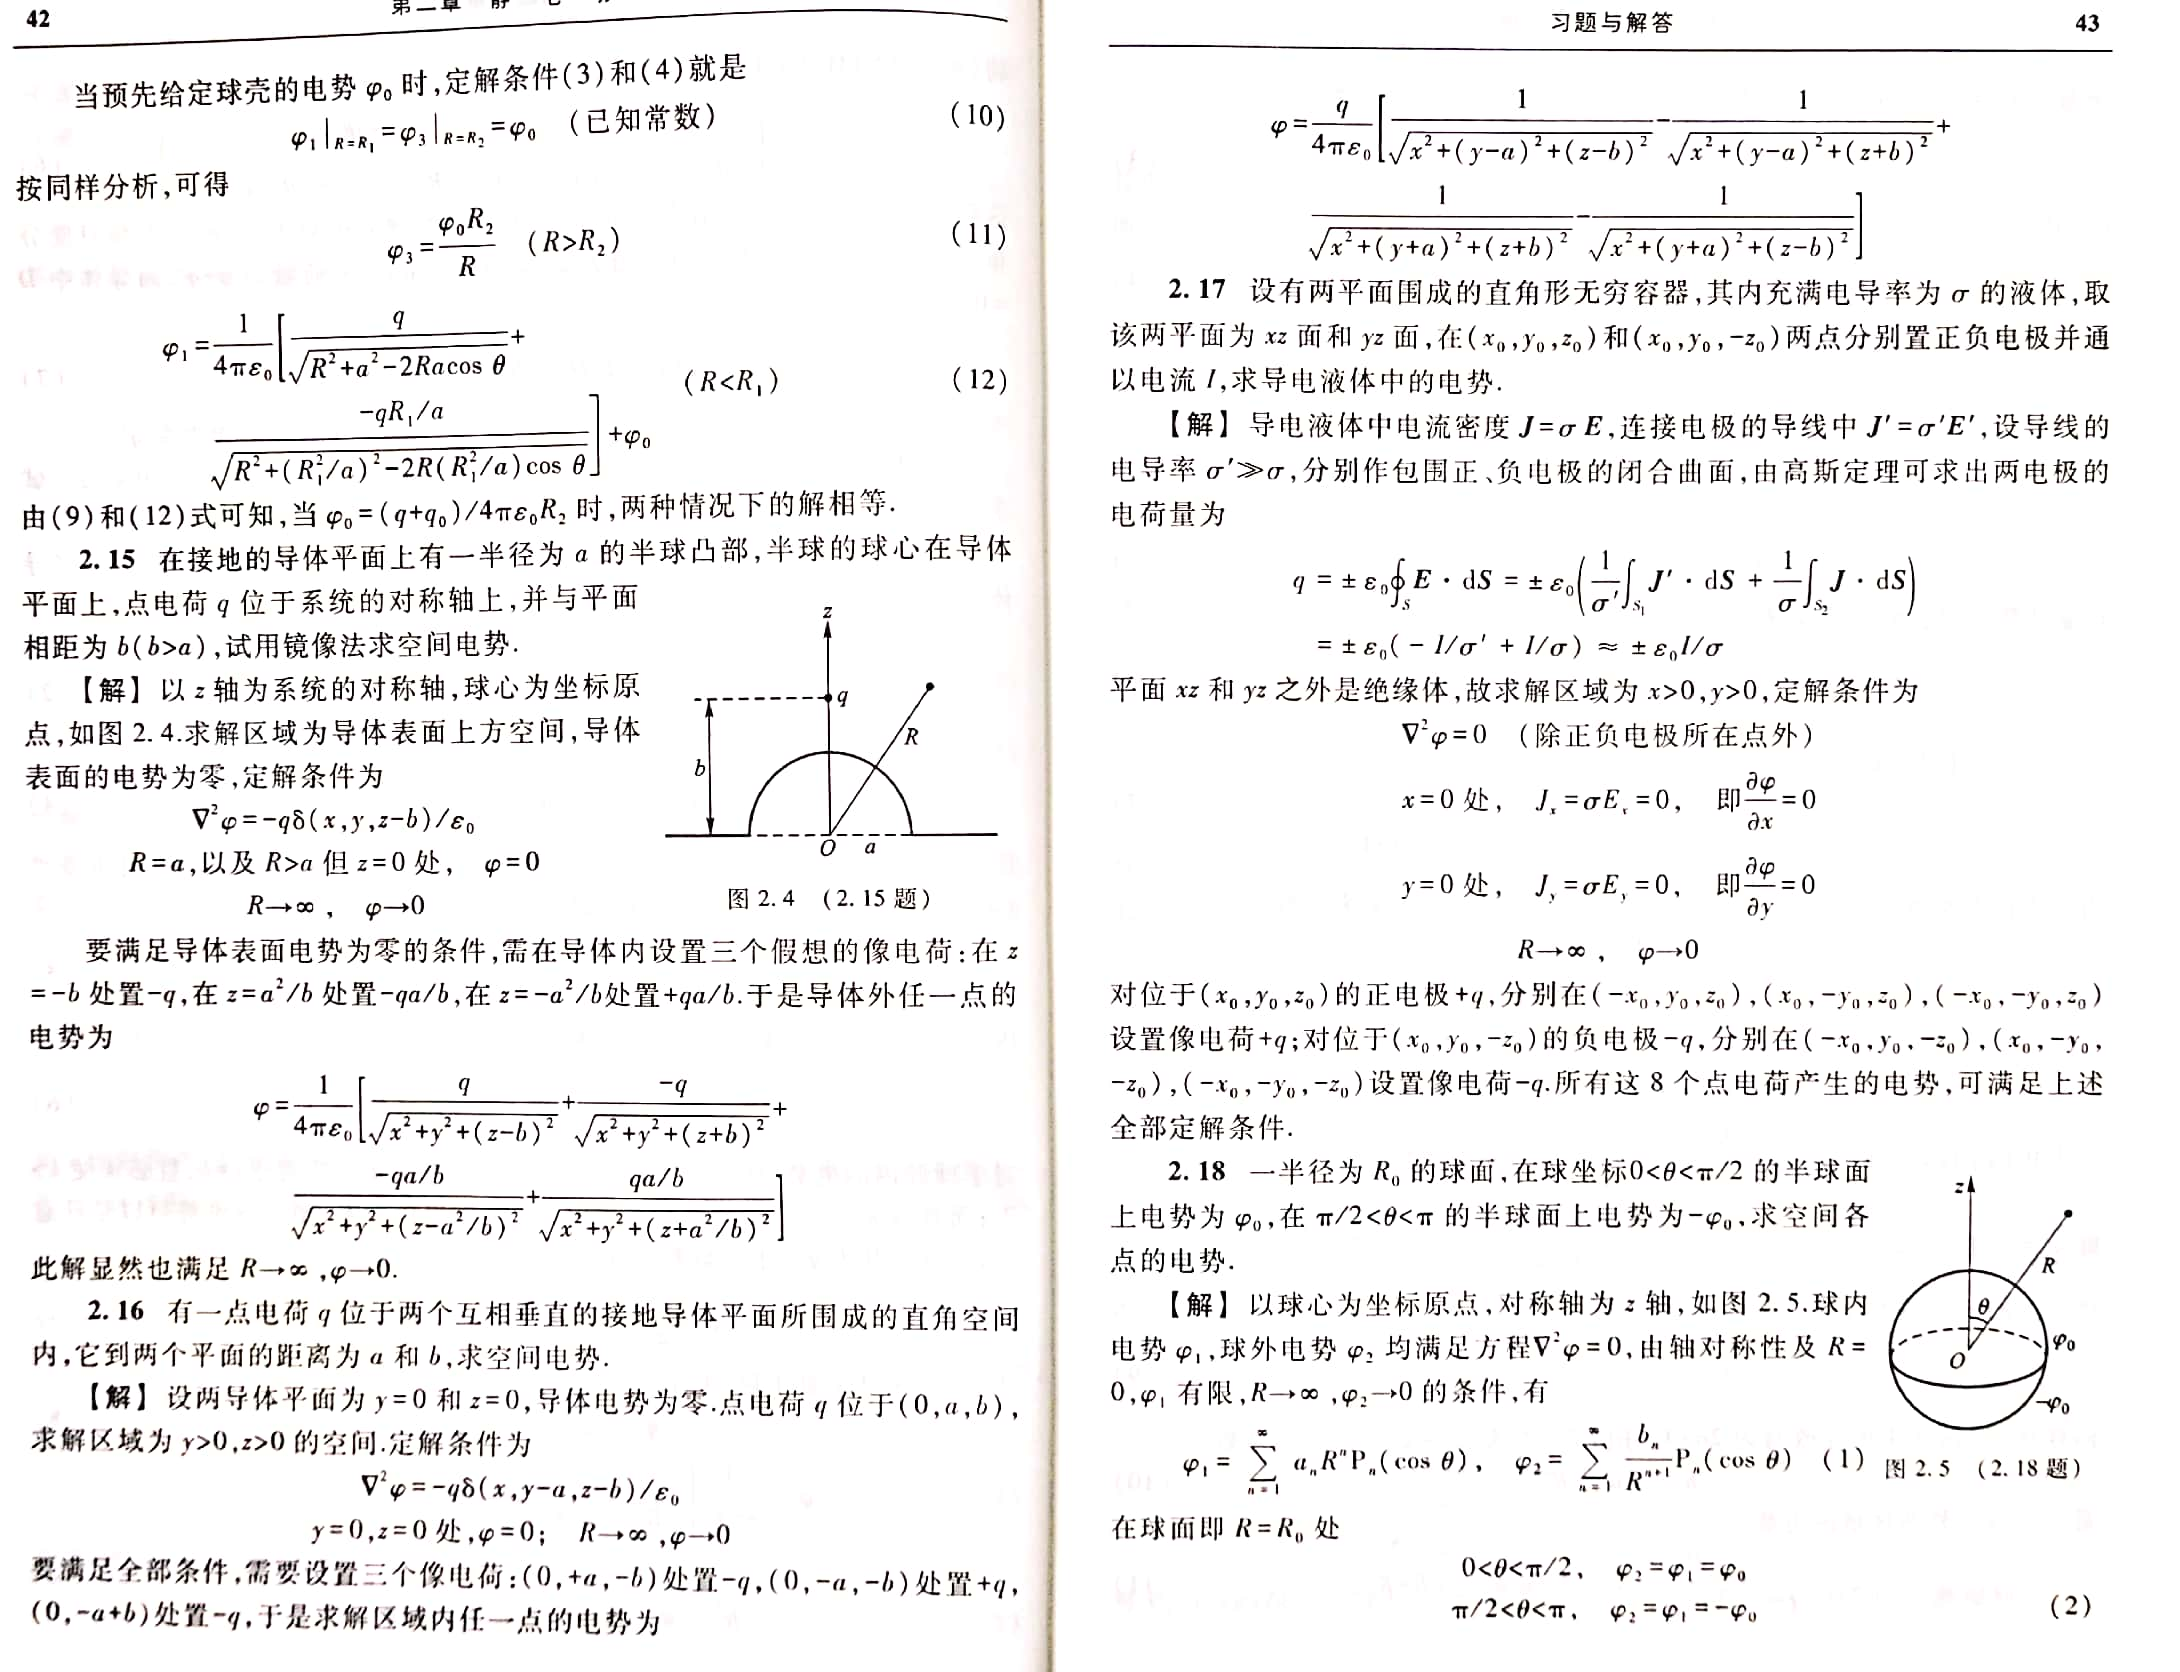
\includegraphics[scale=0.5]{7.jpg}}
    \end{minipage}
    \begin{minipage}[t]{0.48\textwidth}
        \centering
        \boxed{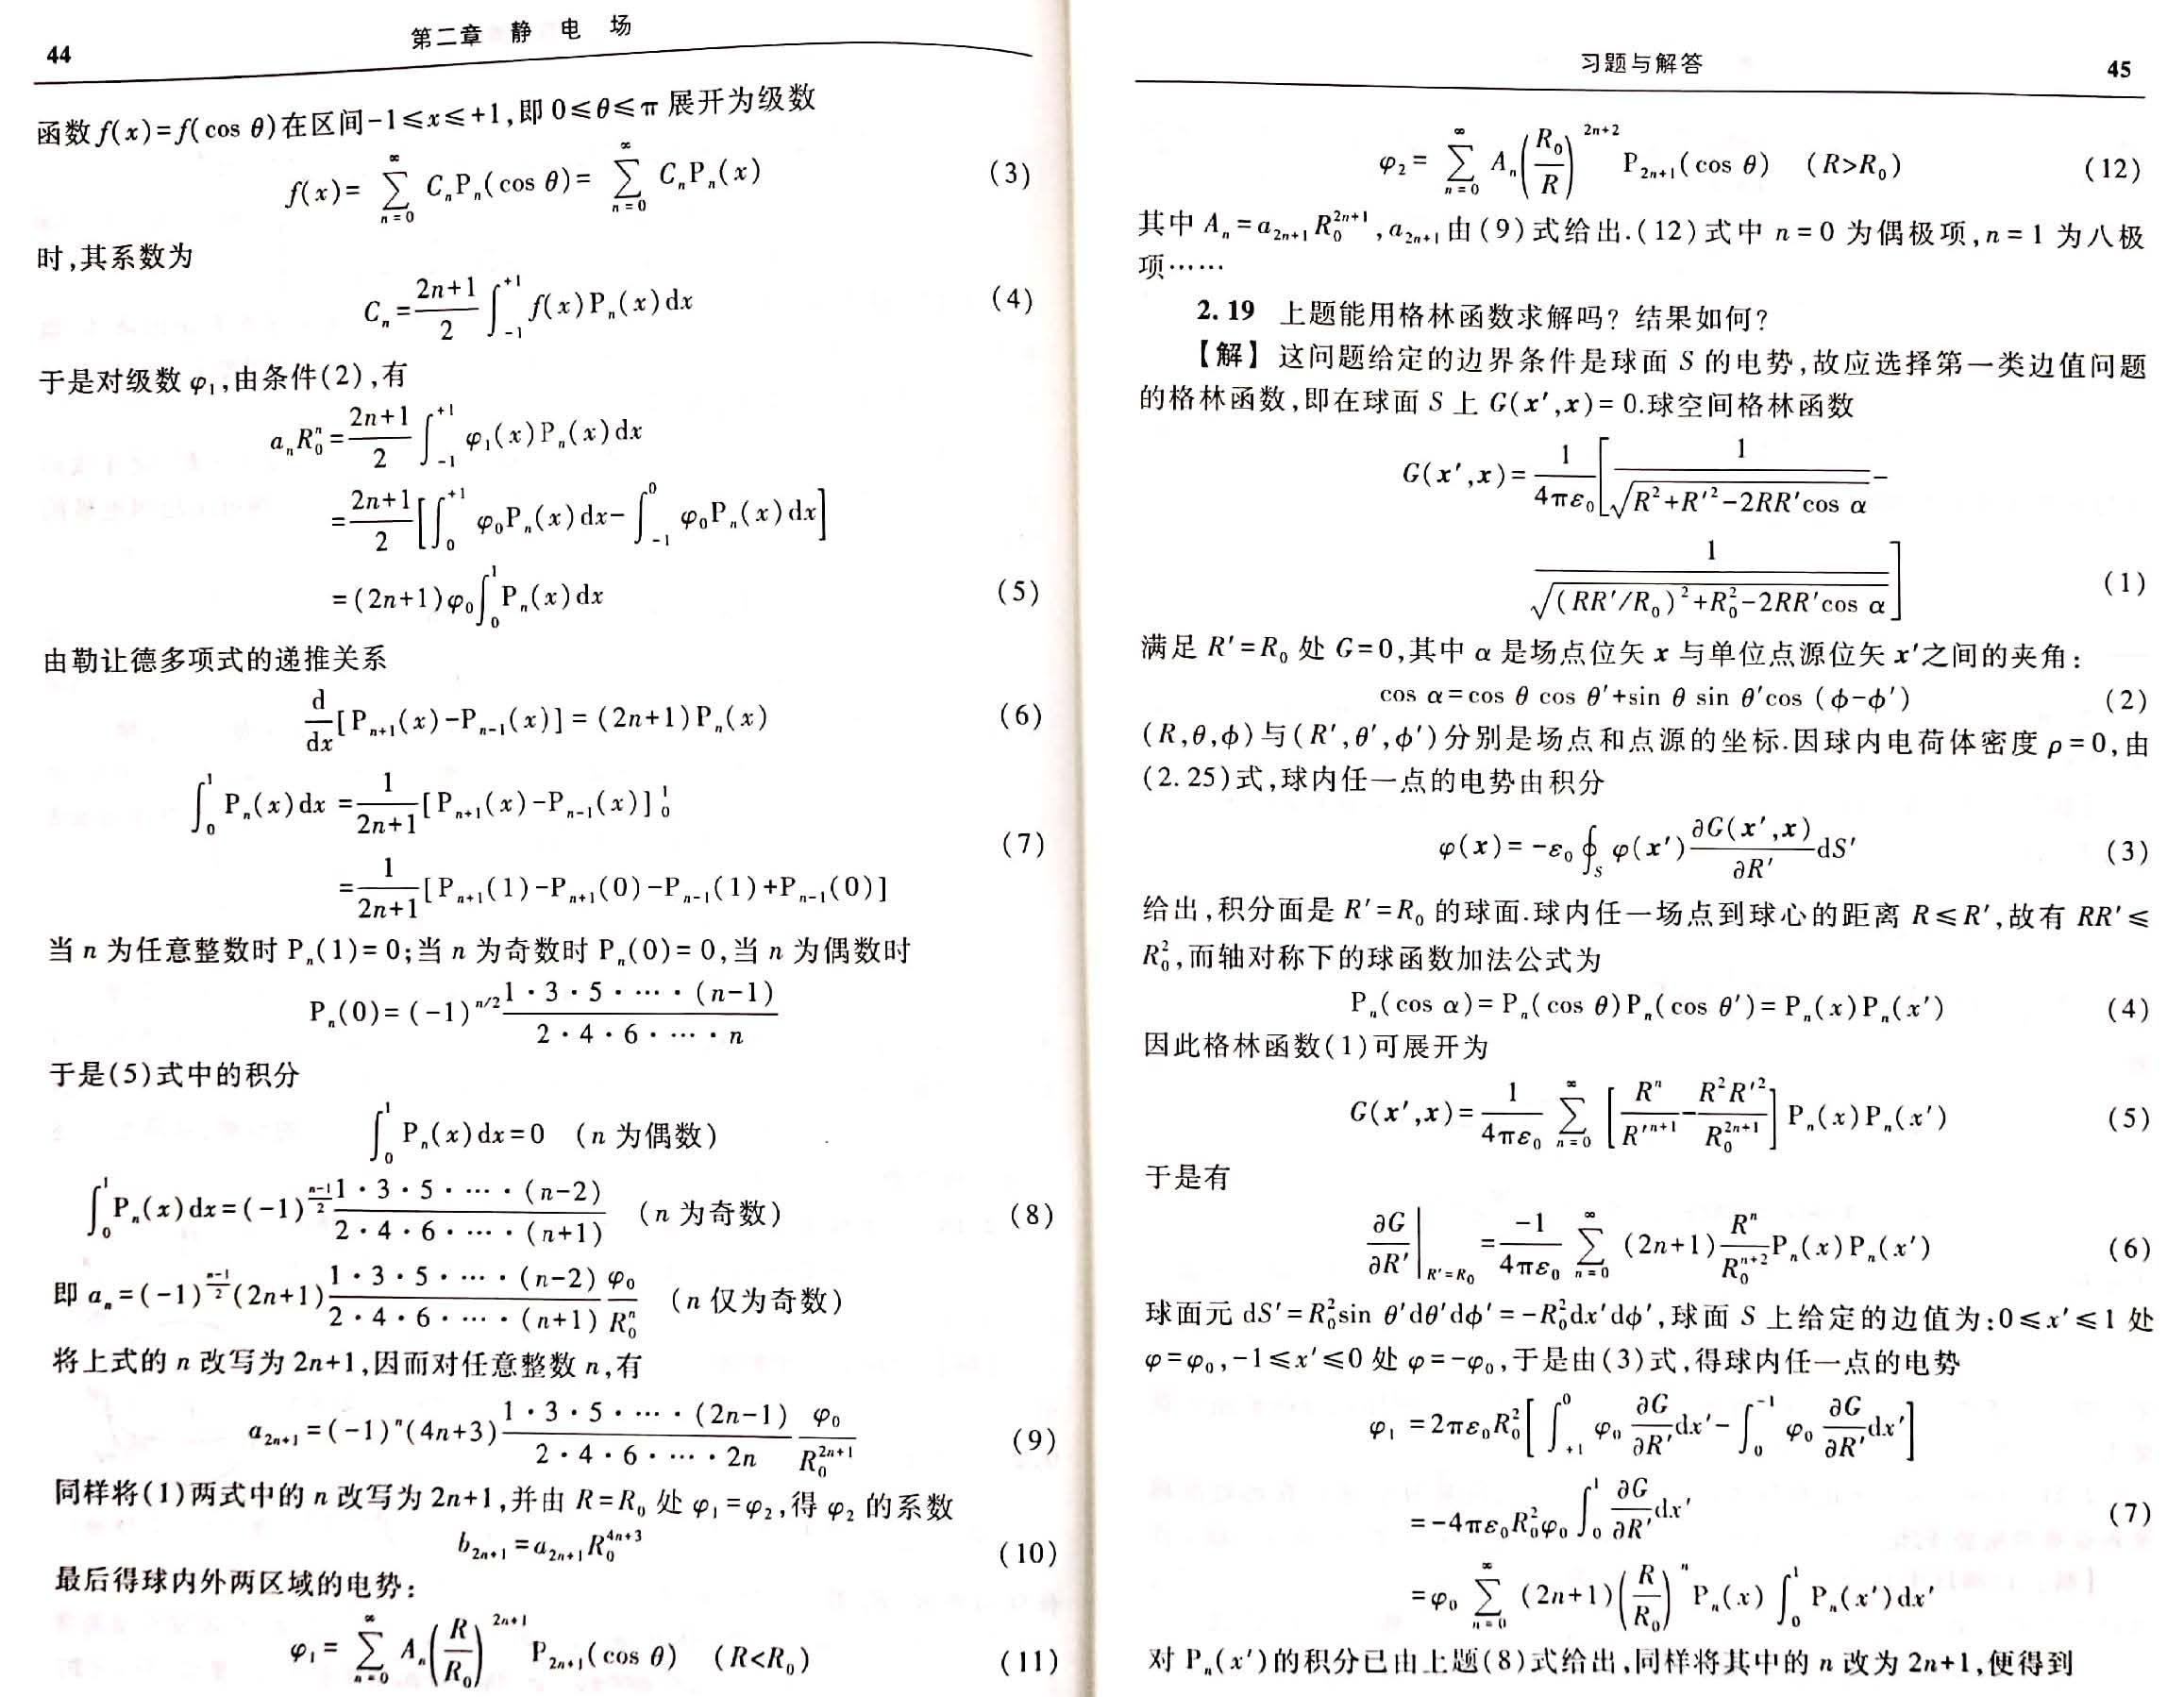
\includegraphics[scale=0.5]{8.jpg}}
    \end{minipage}
\end{figure}
\end{document}